\section{Algorithm} % (fold)

Before taking deep look into the methods, we need to define input and output. The input is pedestal subtracted PMT waveform(Fig \ref{fig:input}), and the output is the charge or penumber sequence(Fig \ref{fig:output}). 

\begin{figure}[H]
\begin{minipage}{.5\textwidth}
\begin{figure}[H]
    \centering
        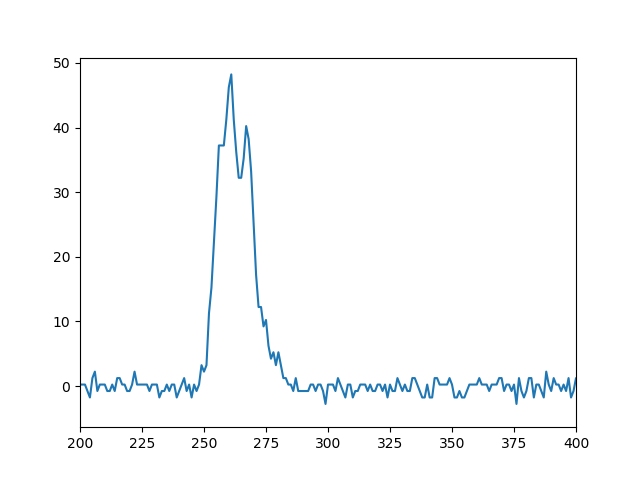
\includegraphics[width=1.0\textwidth]{figures/wave.png}
    \caption{Data input}
    \label{fig:input}
\end{figure}
\end{minipage}
\begin{minipage}{.5\textwidth}
\begin{figure}[H]
    \centering
        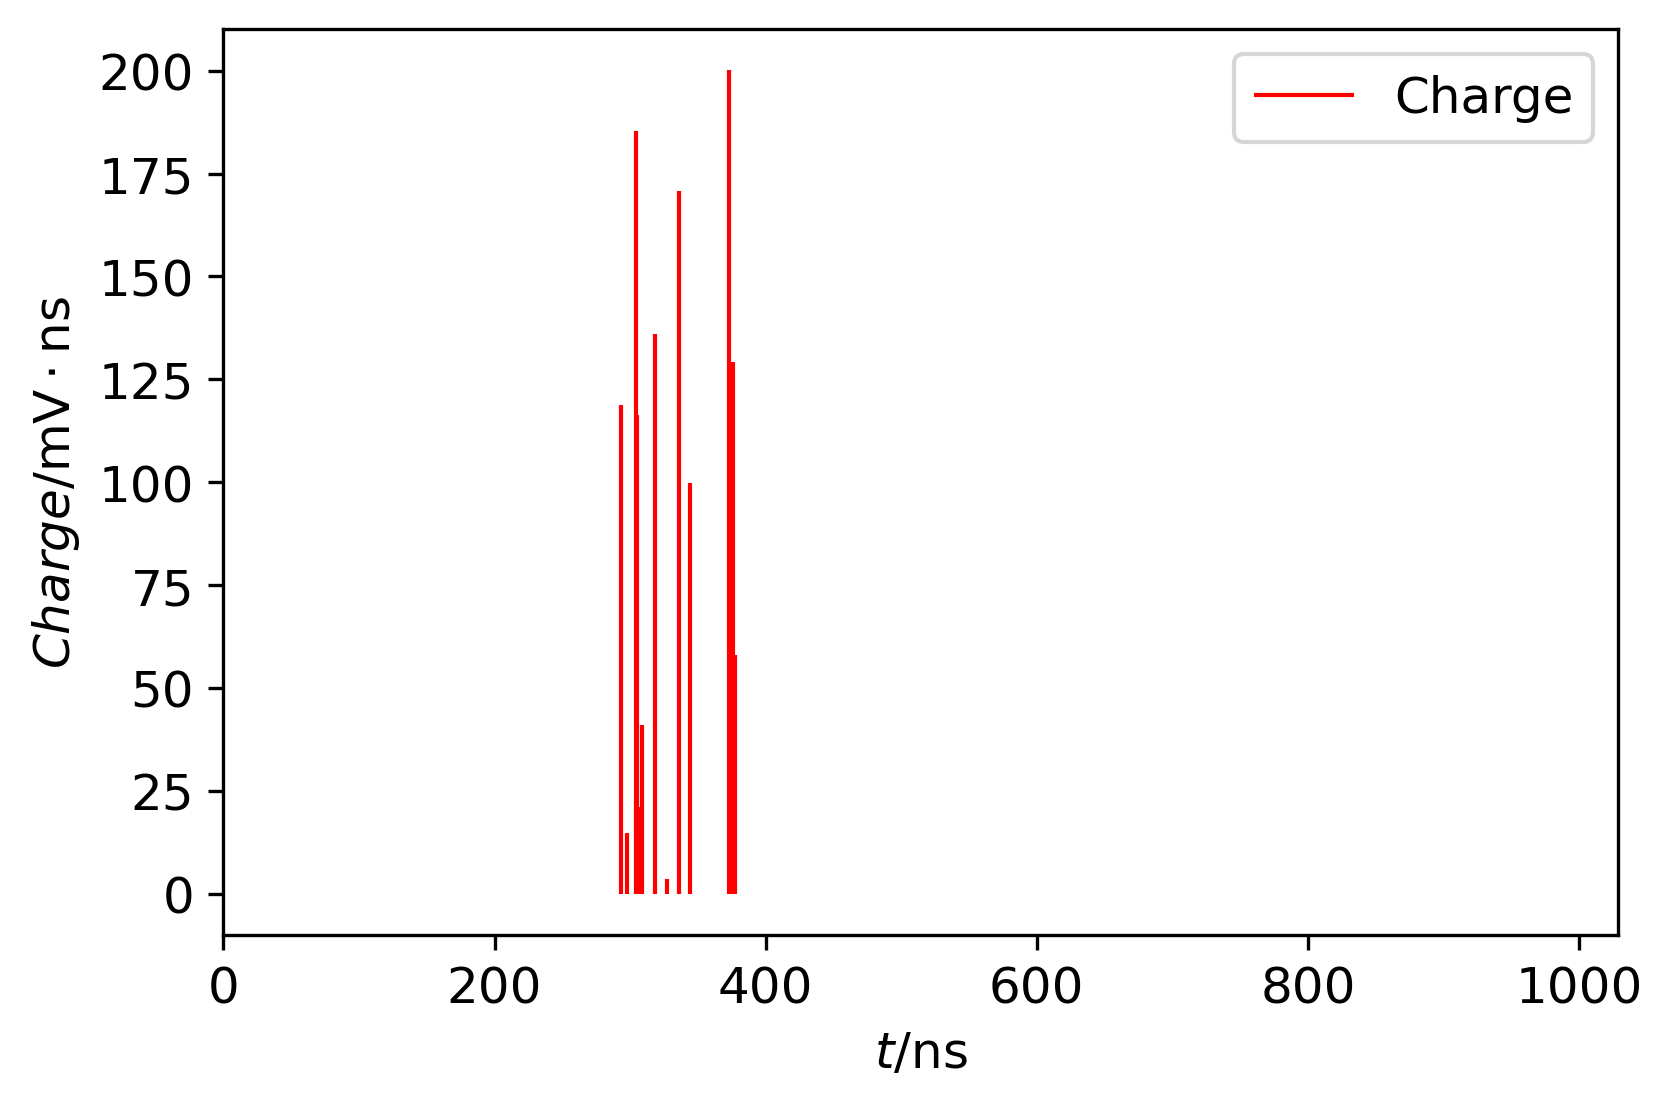
\includegraphics[width=1.0\textwidth]{figures/charge.png}
    \caption{Data output}
    \label{fig:output}
\end{figure}
\end{minipage}
\end{figure}

Total photo-electron number is the count of hittime. The histogram of Total photo-electron number and data structure show in figure(Fig \ref{fig:penum}). 

\begin{figure}[H]
\begin{minipage}{.5\textwidth}
\begin{figure}[H]
    \centering
        \includegraphics[width=1.0\textwidth]{figures/penum.png}
    \caption{TotalPEnum Histogram}
    \label{fig:penum}
\end{figure}
\end{minipage}
\begin{minipage}{.5\textwidth}
\begin{figure}[H]
    \centering
        \includegraphics[width=0.7\textwidth]{figures/dataset.png}
    \caption{Data Structure}
    \label{fig:set}
\end{figure}
\end{minipage}
\end{figure}

\subsection{Find Peak}
First intuitive method is find peak method. First we find the peak of waveform, then we move leftward. The delta t we move is the peak time of single pe response. 

\begin{figure}[H]
    \centering
    \caption{Find Peak Method Demo, W-dist = 4.02}
    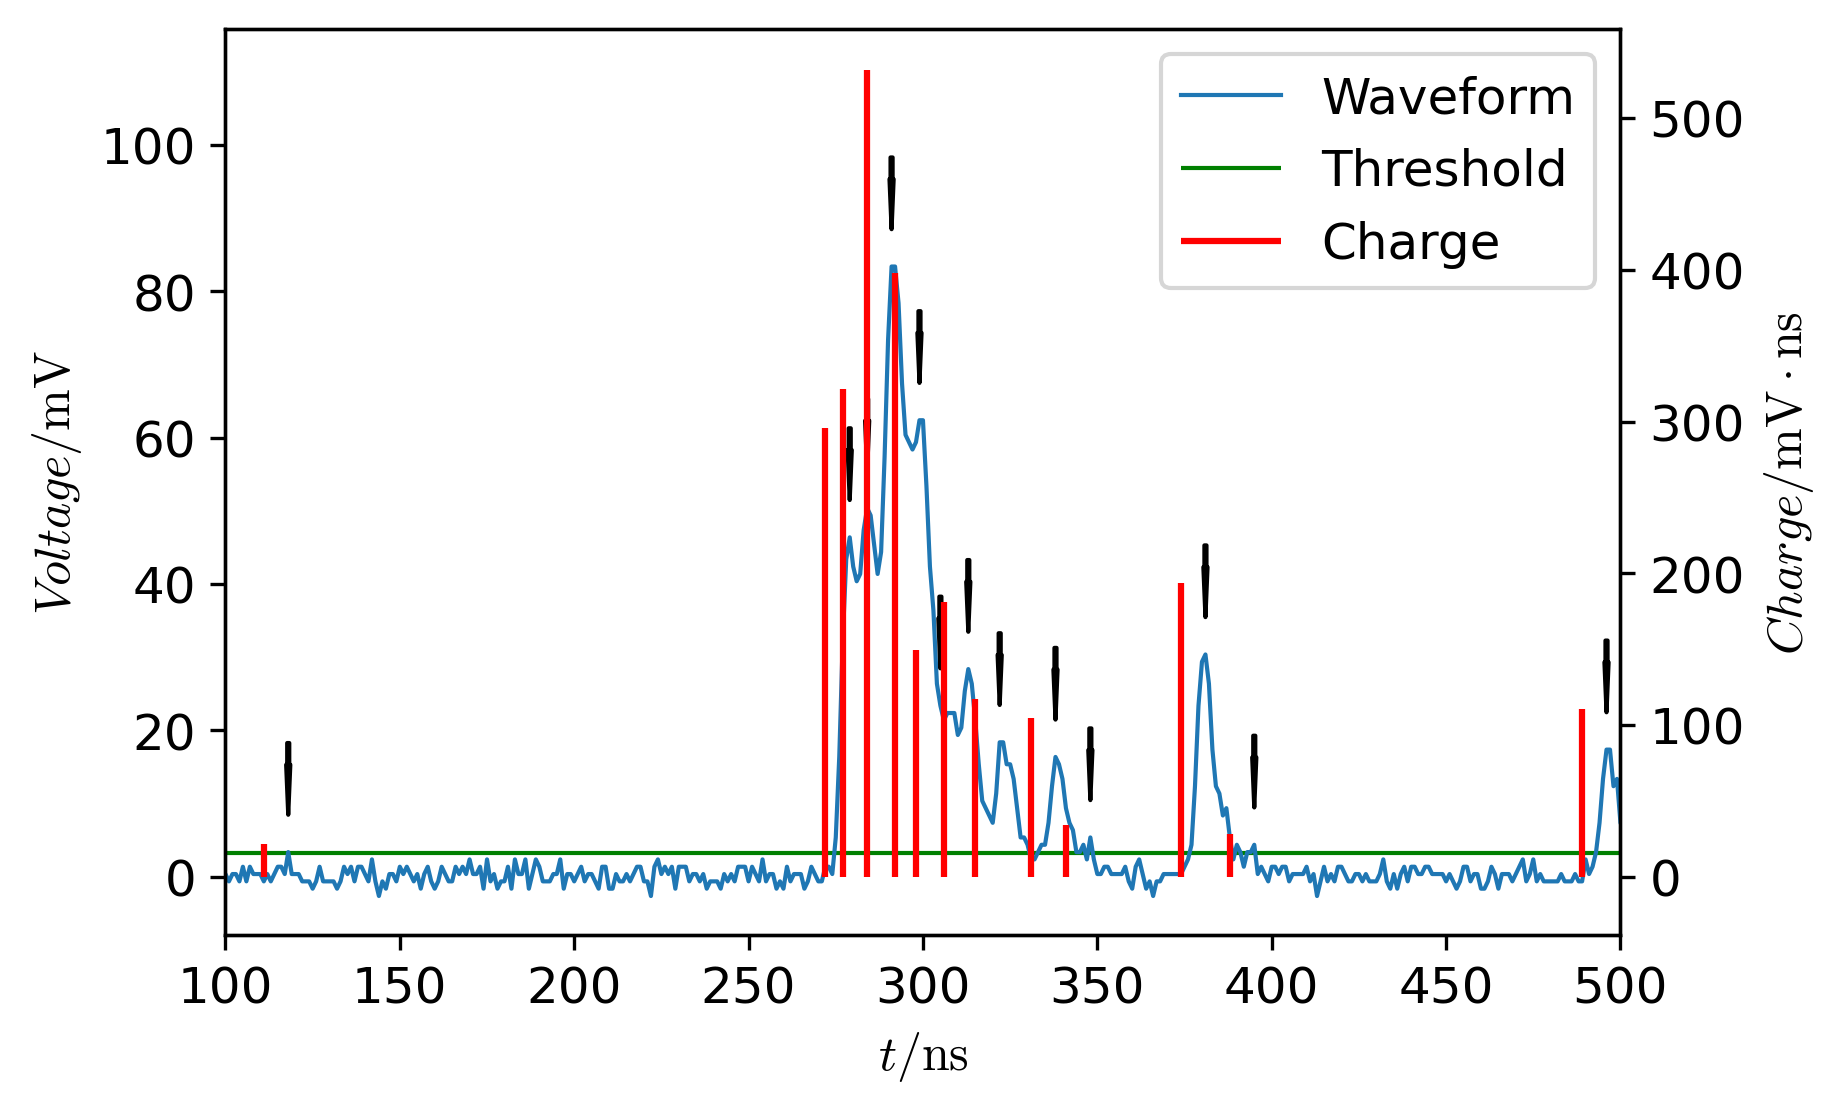
\includegraphics[width=0.6\linewidth]{figures/findpeak.png}
\end{figure}

\subsection{Waveform Shift}
Next is waveform shift method. First we locate the part of waveform exceeds threshold. Then we shift the exceeding part leftward. And treat the normalized exceeding part as charge or penum. 

\begin{figure}[H]
    \centering
    \caption{Waveform Shift Method Demo, W-dist = 10.75}
    \includegraphics[width=0.6\linewidth]{figures/threshold.png}
\end{figure}

\subsection{Fourier Transform Deconvolution}
Third method is Fourier deconvolution. We assume that the waveform is the convolution of single pe response and hittime sequence, so we compute the fft of waveform and single pe response, add a rectangular filter, then compute the inverse fft of the quotient of filtered fft of waveform and fft of single pe response. 

\begin{figure}[H]
    \centering
    \caption{Fourier Deconvolution Demo, W-dist = 1.63}
    \includegraphics[width=0.6\linewidth]{figures/fftrans.png}
\end{figure}

\subsection{Lucy Deconvolution}
Next is Lucy deconvolution. Lucy-Richardson deconvolution is a non linear iteration method, to calculate the deconvolution of signals. Lucy deconvolution has an advantage against Fourier deconvolution. Lucy deconvolution has a constraint that charge or penum are larger than 0. 

\begin{figure}[H]
    \centering
    \caption{Lucy Deconvolution Demo, W-dist = 1.25}
    \includegraphics[width=0.6\linewidth]{figures/lucyddm.png}
\end{figure}

\subsection{Fitting}
First we extract enough single PE response from simulation data. We suppose the average of these waveforms is the single PE response. In fitting process, the parameter is weight in each discrete hittime. The loss which we need to optimize is the truth wave and reconstructed wave according to the parameters. The graph here shows one of the fitting result. We can see the truth waveform and reconstructed waveform is very similar. 

\begin{figure}
    \centering
    \caption{Fitting Demo, W-dist = 1.51}
    \includegraphics[width=0.8\linewidth]{figures/demo.png}
\end{figure}

\begin{figure}[H]
\begin{minipage}{.5\textwidth}
\begin{figure}[H]
    \centering
        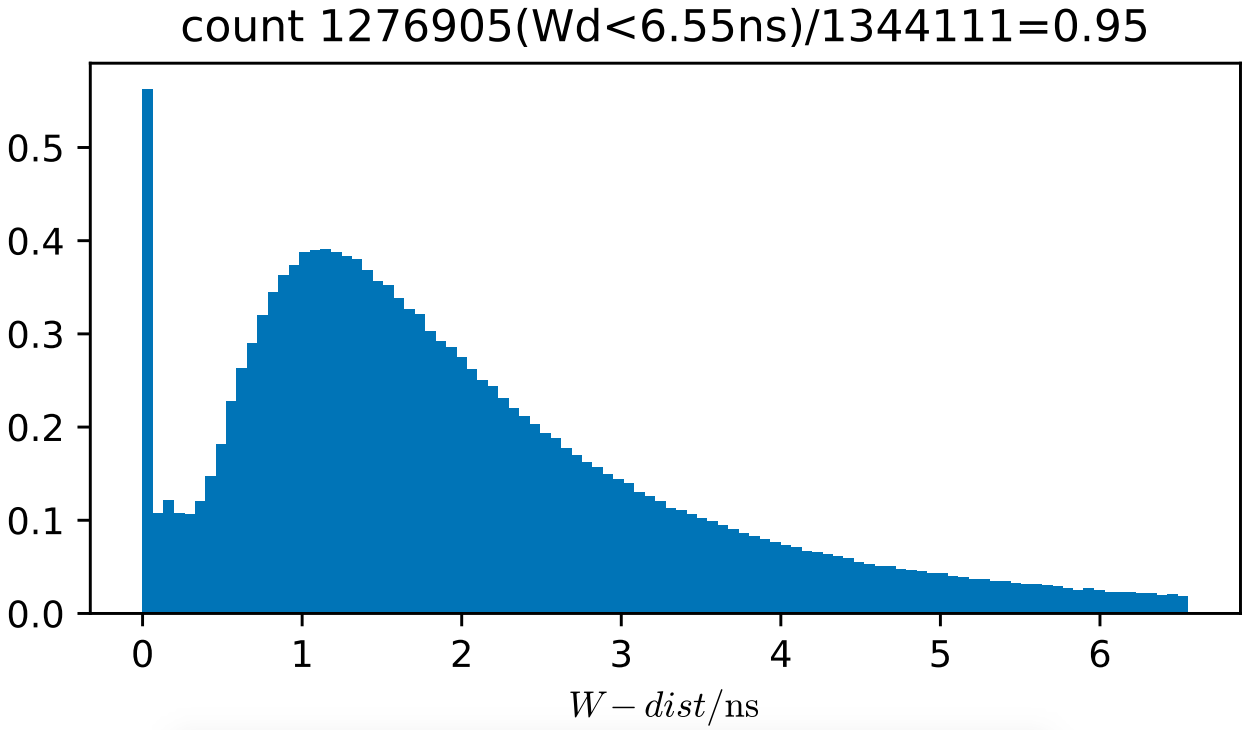
\includegraphics[width=1.0\textwidth]{figures/xiaopeippenumhist.png}
    \caption{Fitting \#PE Result Histogram}
\end{figure}
\end{minipage}
\begin{minipage}{.5\textwidth}
\begin{figure}[H]
    \centering
        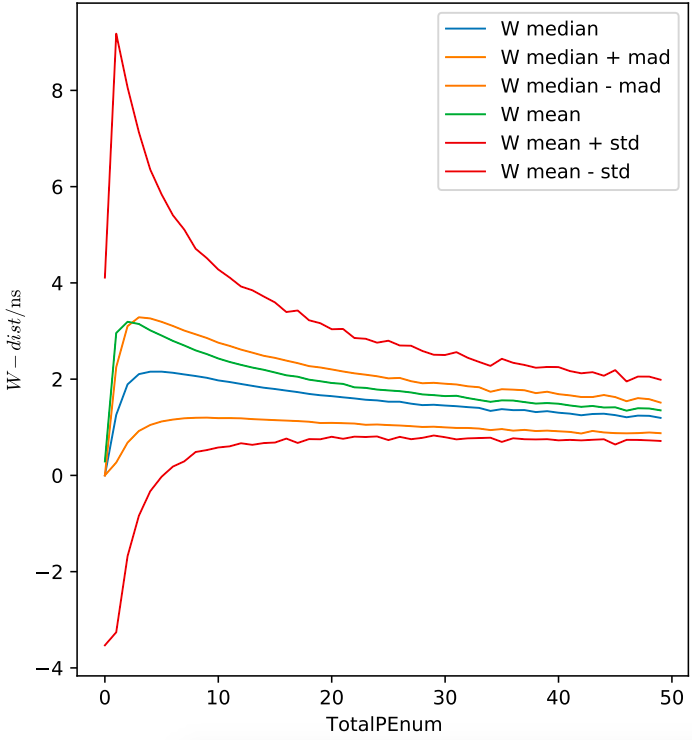
\includegraphics[width=0.7\textwidth]{figures/xiaopeippenumstats.png}
    \caption{Fitting \#PE W-dist vs TotalPEnum}
\end{figure}
\end{minipage}
\end{figure}
\begin{figure}[H]
\begin{minipage}{.5\textwidth}
\begin{figure}[H]
    \centering
        \includegraphics[width=1.0\textwidth]{figures/xiaopeipchargehist.png}
    \caption{Fitting Charge Result Histogram}
\end{figure}
\end{minipage}
\begin{minipage}{.5\textwidth}
\begin{figure}[H]
    \centering
        \includegraphics[width=0.7\textwidth]{figures/xiaopeipchargestats.png}
    \caption{Fitting Charge W-dist vs TotalPEpos}
\end{figure}
\end{minipage}
\end{figure}

\subsection{CNN}
A convolutional neural network is developed to analys the waveform. Here is the structure of CNN which has 5 convolutional layer(Fig \ref{fig:struct}). The length of data remains the same. 

\begin{figure}[H]
\begin{minipage}{.3\textwidth}
\begin{figure}[H]
    \centering
    \caption{CNN Structure}
    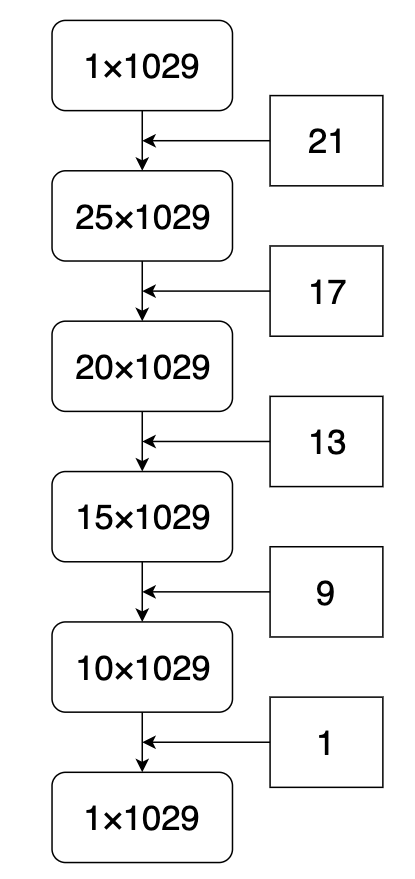
\includegraphics[width=0.8\textwidth]{figures/model.png}
    \label{fig:struct}
\end{figure}
\end{minipage}
\hspace{4mm}
\begin{minipage}{.7\textwidth}
\lstinputlisting[language=Python, basicstyle=\small]{figures/CNN}
\end{minipage}
\end{figure}

In the training process, we trained CNN for each PMT channel. The loss which is Wasserstein distance during training show in Figure \ref{fig:loss}. 

\begin{figure}[H]
    \centering
    \caption{Loss variation during training}
    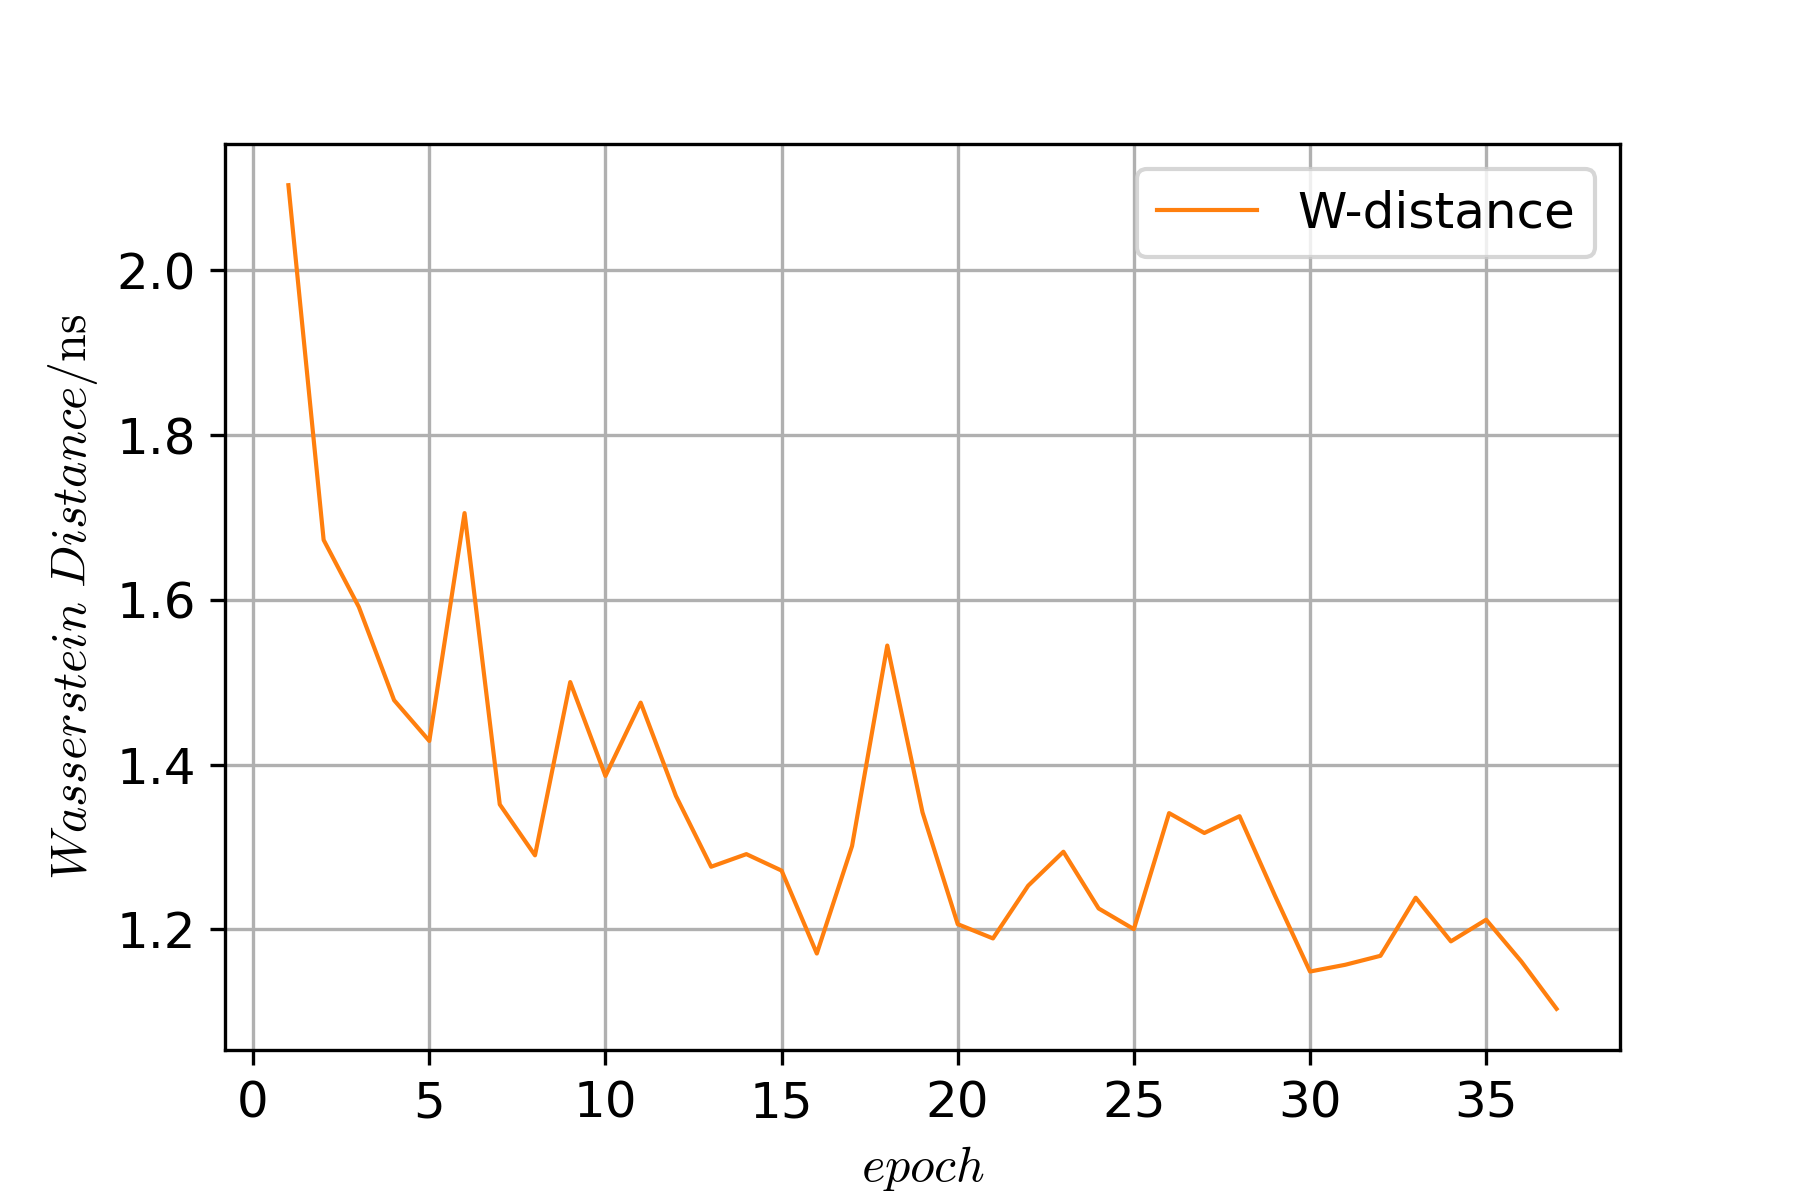
\includegraphics[width=0.6\linewidth]{figures/epoch.png}
    \label{fig:loss}
\end{figure}

The result shows that CNN is the best for reconstruction of Charge and \#PE. 

\begin{figure}[H]
\begin{minipage}{.5\textwidth}
\begin{figure}[H]
    \centering
        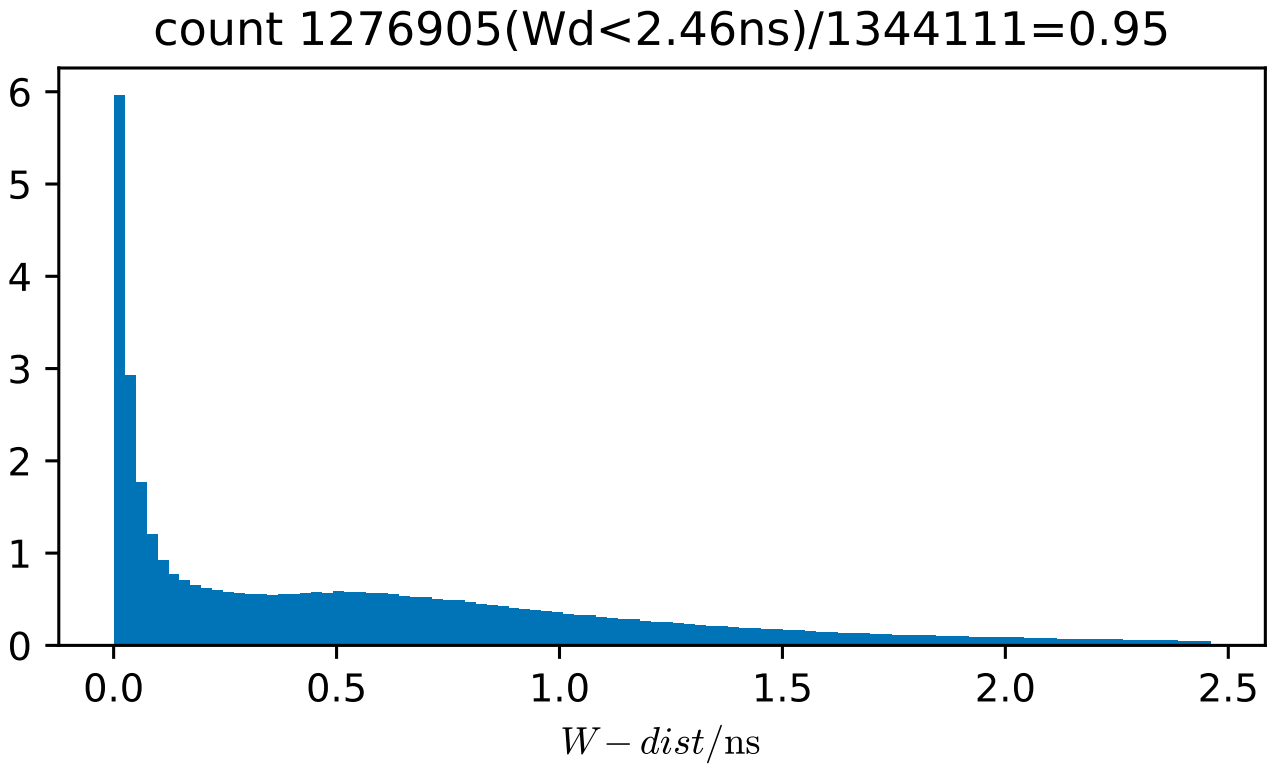
\includegraphics[width=1.0\textwidth]{figures/takarapenumhist.png}
    \caption{CNN \#PE Result Histogram}
\end{figure}
\end{minipage}
\begin{minipage}{.5\textwidth}
\begin{figure}[H]
    \centering
        \includegraphics[width=0.7\textwidth]{figures/takarapenumstats.png}
    \caption{CNN \#PE W-dist vs TotalPEnum}
\end{figure}
\end{minipage}
\end{figure}
\begin{figure}[H]
\begin{minipage}{.5\textwidth}
\begin{figure}[H]
    \centering
        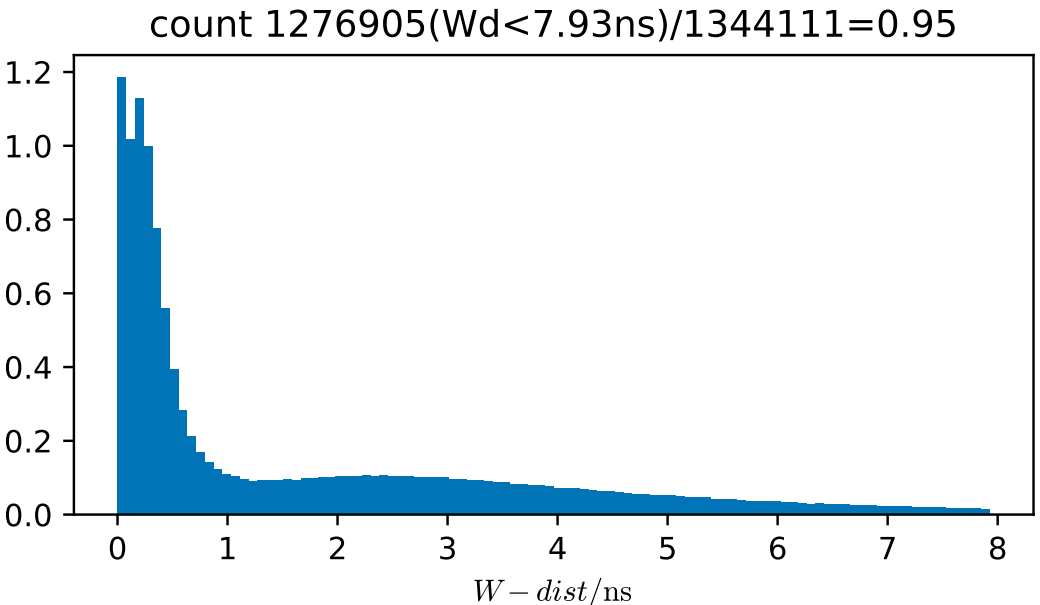
\includegraphics[width=1.0\textwidth]{figures/takarachargehist.png}
    \caption{CNN Charge Result Histogram}
\end{figure}
\end{minipage}
\begin{minipage}{.5\textwidth}
\begin{figure}[H]
    \centering
        \includegraphics[width=0.7\textwidth]{figures/takarachargestats.png}
    \caption{CNN Charge W-dist vs TotalPEpos}
\end{figure}
\end{minipage}
\end{figure}

% section Algorithm (end)